\section{Today's assignment}
Today's class will demystify the Transformer architecture \cite{vaswani2017attention}. Transformers have become the dominant model in Natural Language Processing pushing the performance of all tasks through models like BERT \cite{devlin2018bert} and GPT \cite{brown2020language}. In this class, we will review the architecture of Transformers. The focus of the class is to understand and implement the self-attention mechanism in Pytorch. For this, we will use an annotated version of Karpathy's miniGPT library.


\section{Transformer Architectures}

The basic building block of the Transformer combines a large Feed forward network with a multi-head self-attention layer. We have seen feed forwards in previous days and we will focus here on multi-head self-attention. Refer to previous days for details on the basics of feed-forwards.

Transformer blocks can be found in three types: Encoder, Decoder, and Encoder-Decoder 

\begin{enumerate}
\item Encoders: map a sequence of $T$ observations, e.g. some word or sub-word units $x_1 \cdots x_T$ to a hidden representation of size $H$, yielding a matrix of embeddings of size $(H, T)$. These contextual embeddings can be used to build other models on top by adding extra layers e.g. BERT.
\item Decoders: given a sequence of $t$ observations, e.g. some word or sub-word units $x_{<t} = x_1 \cdots x_{t-1}$ provide a hidden representation for element $x_t$. This can be used to predict the next word given some partial sentence e.g. as in GPT. 
\item Cross-Attention-Decoders: map a sequence $x$ to another of different size $y$. For this, they first Encode $x$ using an encoder. And then use a modified Decoder, that uses an additional attention mechanism read the Encoder values to generate embeddings for $y_t$ given $y_{<t}$ and the $\mathrm{Encoder}(x)$. The original Transformer used for machine translation is the best example.
\end{enumerate}

Though with very different roles the three architectures are very close to each other and imply only minor modifications. We will focus here on the Encoder architecture first, and then we will explain the other two.

\section{Attention}
In this section, we will delve into the intricacies of the attention mechanism, aiming to grasp its underlying intuition and motivation. We will embark on a comprehensive exploration of its inner workings, unraveling its secrets along the way.

Attention mechanisms have become a crucial component in effective sequence modeling across different tasks e.g. Neural Machine Translation (NMT) \cite{vaswani2017attention}. They enable the modeling of relationships between elements in input or output sequences, regardless of their positional distance. \cite{bahdanau2014neural, kim2017structured}.

The state-of-the-art sequence modeling architectures that predate Transformers, such as Recurrent Neural Networks (RNN), have traditionally treated input information in a uniform manner. This means that no specific connections are established among the individual tokens to fully capture the intricate relationships between them. Essentially, each token denoted as $t_i$, receives information from all preceding tokens $t_1...t_{i-1}$ in a uniform fashion. However, as the value of $i$ increases, this approach often leads to information loss, as well as issues related to vanishing or exploding gradients \cite{hochreiter1997long}, due to the fixed dimensionality of the encoded information.

In order to mitigate the latter challenge, Long Short-Term Memory (LSTM) models were introduced. These models proposed mechanisms to manipulate the flow of information across states by selectively adding or removing pertinent and extraneous information \cite{hochreiter1997long}. By incorporating these mechanisms, LSTM models aimed to address the aforementioned issues and enhance the handling of information within the sequence.
The LSTM has demonstrated exceptional performance on challenging sequence prediction tasks, such as text translation, and swiftly emerged as the prevailing approach in the field \cite{cho2014learning, sutskever2014sequence}.

However, the issue of having a fixed-length internal representation persists, and to overcome this limitation in the encoder-decoder architecture, the Attention mechanism was introduced. The Attention mechanism offers various variants, and in this context, we will delve into the "Scaled Dot-Product Attention" as outlined in \cite{vaswani2017attention}.

To provide a practical demonstration of the complex relationships that the model needs to learn, let's consider the following example: \emph{``The cat didn't climb the tree because it was too scared.``}.
\begin{figure}[h]
    \centering
    
\includegraphics[width=8cm]{pages/imgs/example.png}
    \caption{An example illustration}
    \label{fig:example}
\end{figure}
In the initial part of the example, the inner connections are relatively straightforward. However, in the subsequent segment starting from the word "because," the relationships become more intricate.
For a human being, the question of whether the pronoun "it" refers to the cat or the tree is relatively simple due to our prior knowledge about cats and trees. With our understanding of these concepts, we can confidently determine the intended reference of the word "it." 
However, for a model, discerning the referent of the pronoun "it" -- whether it pertains to the cat or the tree -- is not as straightforward. Therefore, we require a mechanism that does not treat all words with equal importance but rather allocates focus to different tokens.

This intuitive mechanism is known as Attention, which assigns significance to specific tokens for a selected token. In Figure \ref{fig:att_self_sample}, the attention mapping of our example is demonstrated. This is commonly referred to as Self-Attention, as the connections are attained at the internal level, i.e. between input tokens.

\begin{figure}[h]
    \centering
    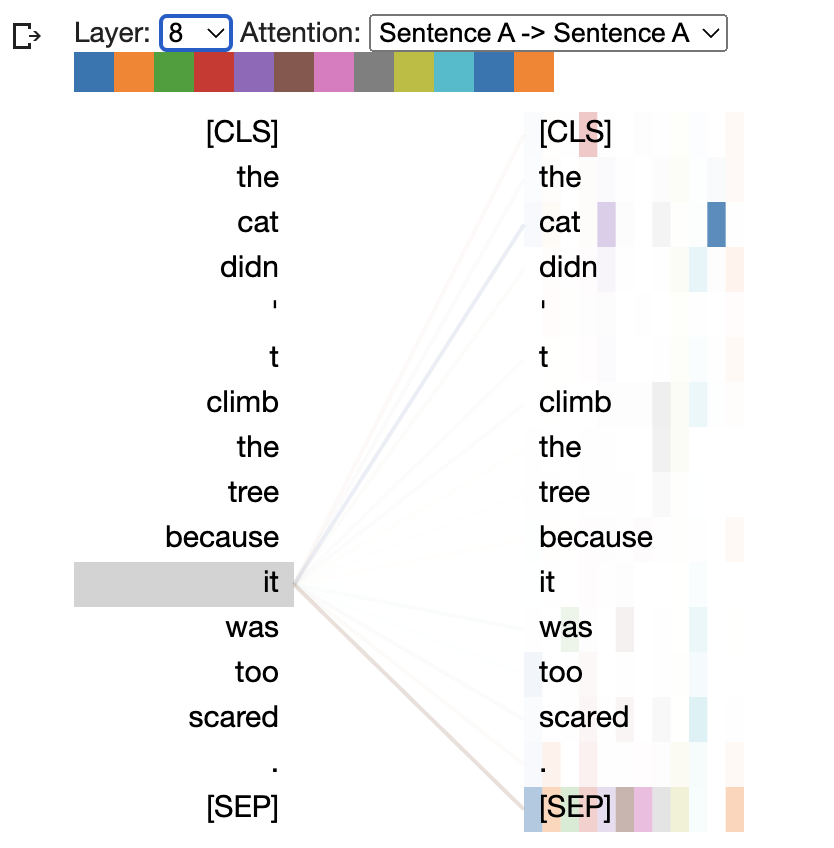
\includegraphics[width=8cm]{pages/imgs/att_self_sample.png}
    \caption{Self-Attention of the sample}
    \label{fig:att_self_sample}
\end{figure}

Capturing the connections between an input and an output sequence is vital for downstream tasks, like Neural Machine Translation (NMT). In this case, the Encoder-Decoder attention mechanism operates in a manner similar to Self-Attention. Let's translate our sample sentence into Portuguese and explore the significant connections it reveals. To accomplish this, we will utilize a pre-trained language model called Multilingual BERT (mBERT), which has knowledge about multiple languages, including English and Portuguese \cite{devlin2018bert}.


\begin{figure}[h]
    \centering
    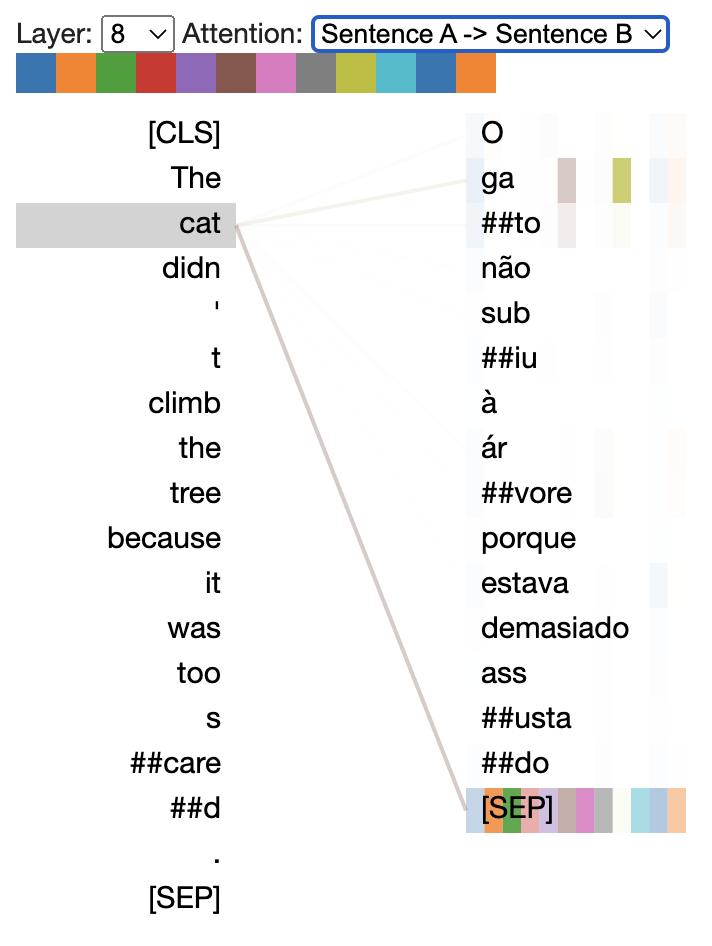
\includegraphics[width=8cm]{pages/imgs/att_cat_sample.png}
    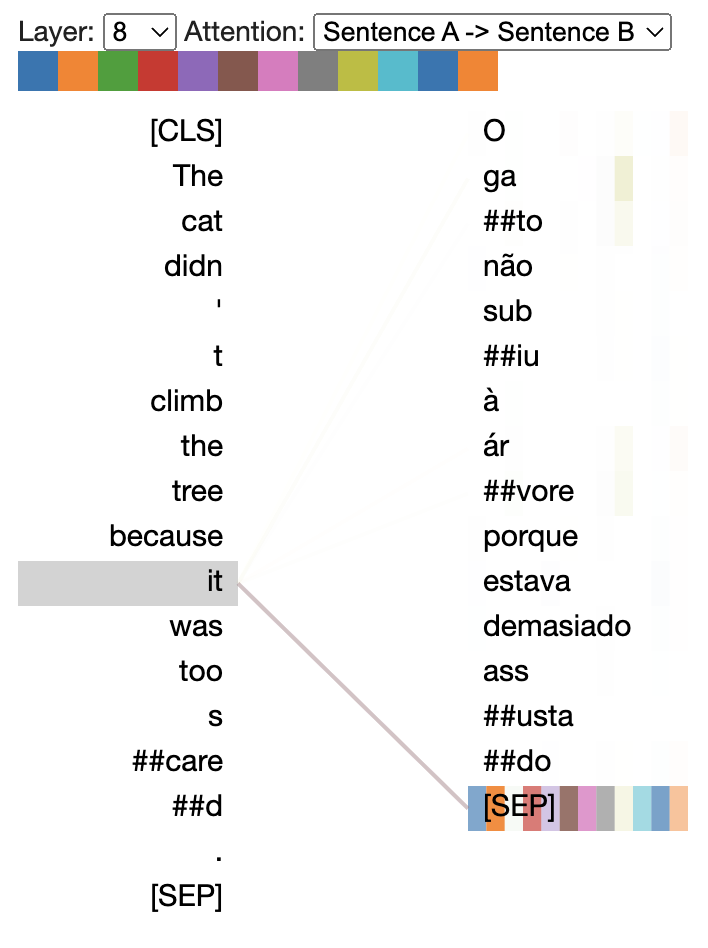
\includegraphics[width=8cm]{pages/imgs/att_it_sample.png}
    \caption{Encoder-Decoder Attention of the sample}
    \label{fig:ed_att_sample}
\end{figure}

In the left image of Figure \ref{fig:ed_att_sample}, we can clearly see that the attention of the token 'cat' is specifically directed towards the token 'gato,' which corresponds to its accurate translation. Similarly, in the right image, the word 'it' is attentively aligned with the token 'gato' once again. These observations indicate the system's ability to effectively focus on the appropriate tokens, both in correctly selecting the appropriate translation, and accurately identifying the relevant noun.

Now let's explore each building block of the Transformer architecture and examine how the Attention mechanism fits in this.



\section{Encoder Architecture}

\subsection{Simplified Encoder Architecture}

the encoder architecture can be succinctly described as stacking a number of $N$ blocks on top of each other combining a feed-forward $\mathrm{FF}$ and Multi-Head Attention $\mathrm{MHA}$ sub-blocks. A single block is defined as

\begin{equation}
e^{n+1} = \mathrm{FF}(\mathrm(MHA(e^n)).
\end{equation}

The input to the first block $e^0$ is the sum of position $P$ and non-contextual embeddings $E$ of the input. Assuming $x_1 \cdots x_T$ is a sequence of integers (indices to a vocabulary of $V$ symbols) we have that

\begin{equation}
e^{0}_t = \mathrm{E} \cdot \mathrm{1}_{x_t} + \mathrm{P} \cdot \mathrm{1}_t \quad \mbox{for} \quad t=1 \cdots T
\end{equation}

where $\mathrm{1}_{x_t}$ and $\mathrm{1}_t$ are indicators, i.e. one-hot, vectors for the token content (vocabulary symbol) and the token position. $\mathrm{E} \in \mathbb{R}^{H \times V}$ is the non-contextual embedding matrix for each symbol in the vocabulary and $P^{H \times \tau}$ is the position embedding matrix, where  $\tau-1$ is the furthest position supported. See Figure \ref{fig:e0} for information flow. \\


\begin{figure}[h]
    \centering
    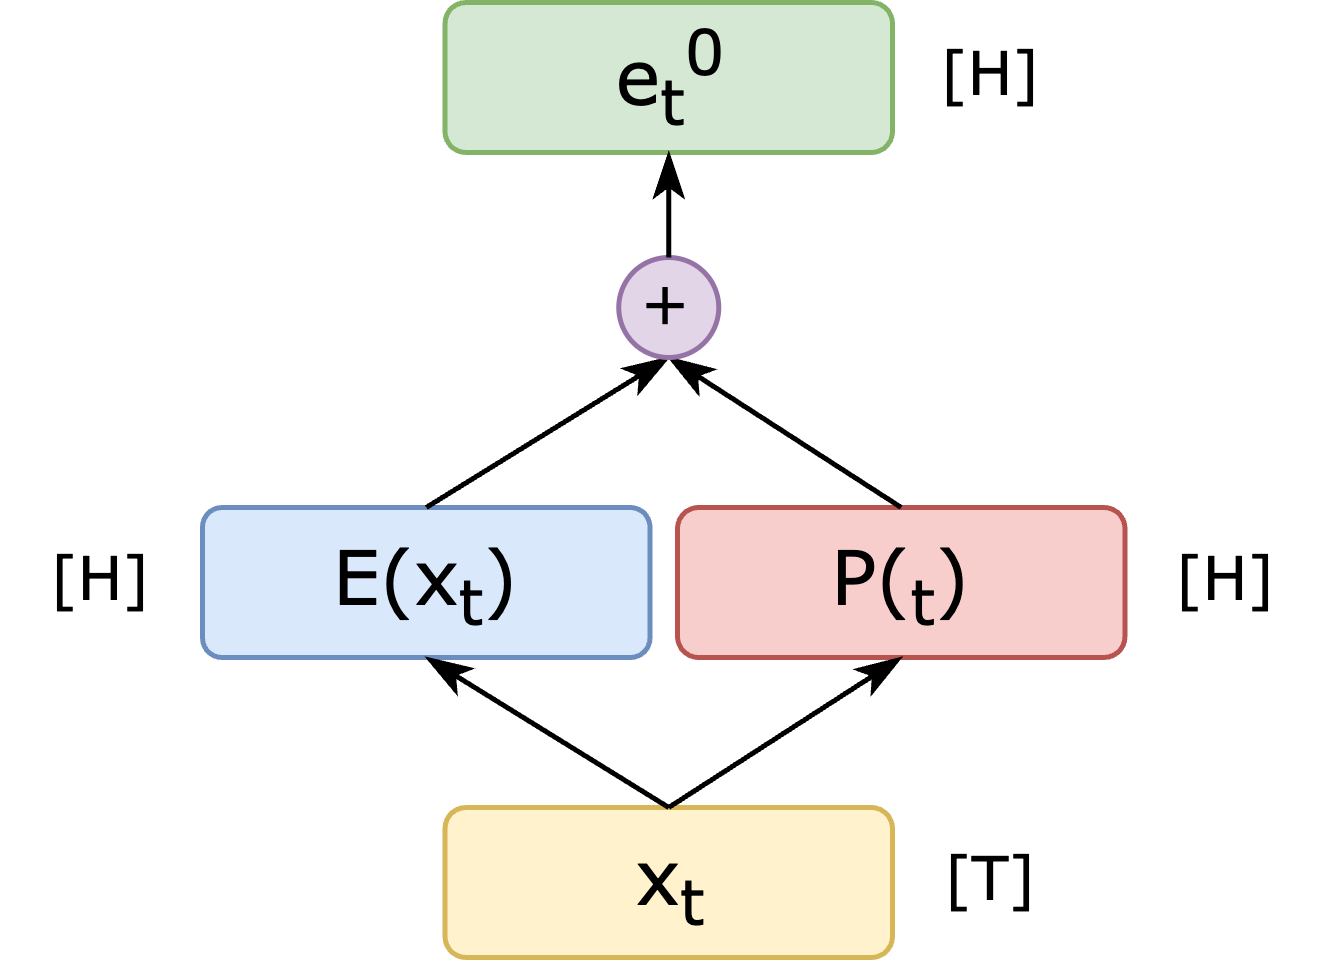
\includegraphics[width=6cm]{pages/imgs/e0.png}
    \caption{Information flow of $t$-th token in layer $e^0$}
    \label{fig:e0}
\end{figure}



\noindent The feed-forward ($\mathrm{FF}$) is given by:

\begin{equation}
FF(z) = W^2\cdot \mathrm{gelu}(W^1 \cdot z)
\end{equation}

\noindent with weight matrices $W^2 \in \mathbb{R}^{H \times 4H}$ and $W^1 \in \mathbb{R}^{4H \times H}$, that expand and contract the hidden dimension $H$.

The Self-Attention ($\mathrm{SA}$) comprises three matrices extracted from the encoder’s input $z$. So, for every given input $z$, we generate a Key vector($K$), a Query vector($Q$), and a Value vector($V$). These matrices are obtained by performing matrix multiplication between the embedding and the corresponding matrix that was learned in the training process, e.g. $Q = W^Q z$.

The next step is to calculate the self-attention score. The Key and Query matrices are multiplied by each other and normalized by a constant value $\frac{1}{A} \left(W^K z\right)^T W^Q z$ or $\frac{1}{A} K^T Q$. The $A$ is usually chosen to be the square root of the dimension of the key matrices. This leads to having more stable gradients.

\noindent Then pass the result through a $softmax$ operation. The Softmax normalizes the scores so they’re all positive and add up to 1. In other words, extracts a distribution of relative scores from a given token for each token in the input sequence.

\noindent After this multiply the output by the Value matrix: $W^V \cdot z \cdot \underset{i \rightarrow}{\mathrm{softmax}}\left( \frac{1}{A} \left(W^K z\right)^T W^Q z \right)$ or simply $V \cdot \underset{i \rightarrow}{\mathrm{softmax}}\left( \frac{1}{A} \left(K \right)^T Q \right)$.

The Multi-Head Attention ($\mathrm{MHA}$) enhances the Self-Attention layer in two ways: it allows the model to focus on different positions within the input, enabling a better understanding of pronoun references; and allowing projection of input embeddings into distinct representation subspaces, thereby improving overall performance.

\noindent Finally getting the following mathematical form for the $\mathrm{MHA}$:


\begin{equation}
MHA(z) =  W^o \cdot
\begin{bmatrix}
    W^V_1 \cdot z \cdot \underset{i \rightarrow}{\mathrm{softmax}}\left( \frac{1}{A} \left(W^K_1 z\right)^T W^Q_1 z \right)\\
    W^V_2 \cdot z \cdot \underset{i \rightarrow}{\mathrm{softmax}}\left( \frac{1}{A} \left(W^K_2 z\right)^T W^Q_2 z \right)\\
    \cdots\\
    W^V_D \cdot z \cdot \underset{i \rightarrow}{\mathrm{softmax}}\left( \frac{1}{A} \left(W^K_D z\right)^T W^Q_D z \right)\\
\end{bmatrix}\nonumber
\end{equation}

where we have $D$ attention heads. Each head contracts the hidden dimension $W^K, W^Q, W^V \in \mathbb{R}^{H / D \times H}$ into a space of size $H / D$ (this has practical implementation consequences). Outputs of all heads are concatenated and projected again with $W^o \in \mathbb{R}^{H \times H}$.

\subsection{Adding Dropout, Layer Normalization, and Residuals}

For simplicity, we have left several additional operations that can be added as a wrapper around $\mathrm{FF}$ and $\mathrm{MHA}$ operations. These can be expressed as

\begin{equation}
C(f)(x) = x + \mathrm{dropout}(f(\mathrm{layernorm}(x)))
\end{equation}

where $f = \{\mathrm{FF}, \mathrm{MHA}\}$.

\subsection{Training with Encoders}


\section{Decoder Architecture}

This is identical to the Encoder architecture with two differences

\begin{enumerate}
    \item We feed if a partial sequence $x_{<t}$ and take the last output $h_{t-1}$ as the hidden vector for $x_t$
    \item We mask every head of $\mathrm{MHA}$ to prevent any value of time $p$ to depend on values of $>p$
\end{enumerate}

The implementation of training realizes 1) by masking input partial sequence $x_{<t}$ and hidden units from the corresponding positions with an attention mask. This attention mask is also applied during inference time. Note that you can obtain the attention mask by calling its field of input\_ids from huggingface.

\subsection{Training with Decoders}

\section{Encoder-Decoder Architecture}

We need two modifications
\begin{enumerate}
    \item Encode the input with an encoder $e^N = \mathrm{Encoder}(x)$
    \item Modify self-attention to use a second query input to be projected with $W^Q$ while the other two project $E^N$ $d^{m+1} = \mathrm{FF}(\mathrm(CMHA(e^N, MHA(d^m))).$
\end{enumerate}

\subsection{Training with Encoder-Decoder}

\section{Misc}
Different from models with recurrence/convolution, positional information is not encoded in Transformers. Therefore, \citet{vaswani2017attention} include the positional embedding as part of the input to Transformers. The most popular way to compute the positional embedding is to use the sinusoidal shown below.
\begin{equation*}
        PE_{(pos,2i)} = sin(pos / 10000^{2i/\dmodel}) \\
        PE_{(pos,2i+1)} = cos(pos / 10000^{2i/\dmodel}),
\end{equation*}

In the assignment, you will also need to write the sinusoidal embedding (this will be changed according to the design of assignments)


\begin{enumerate}
\end{enumerate}

